
\section{Results}


\subsection{Effect of spatial structure in PD and HD games}

In our first simulation experiment, we compared the effect of spatial structure on the persistence of cooperators in the PD and HD games.


(figure \ref{fig: task1_4plot})



\begin{figure}[H]
	\centering 
	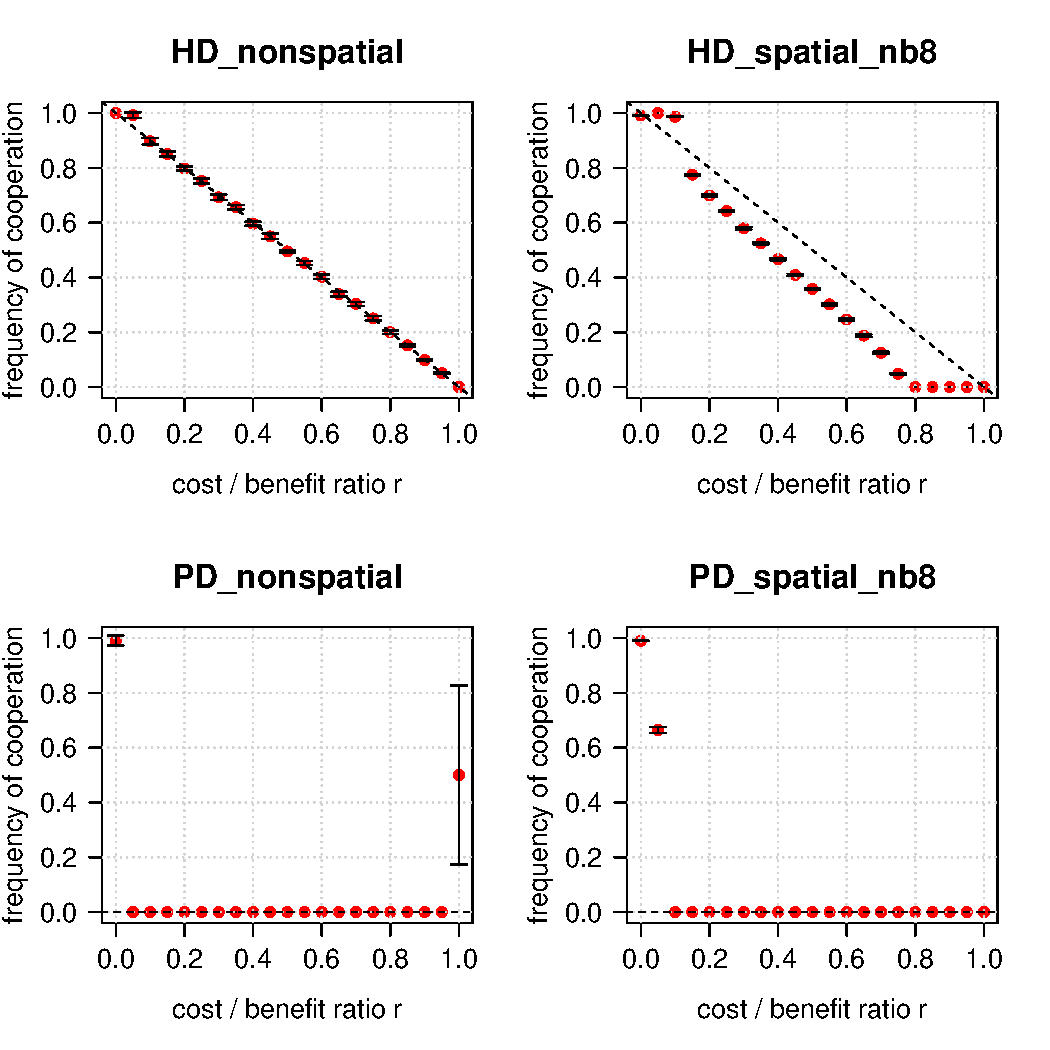
\includegraphics[width=9.5cm]{task1_4plot}
	\caption{Comparison of HD and PD game simulations, both with and without spatial structure.  \textbf{[ t = 5000, i = 10 ]} }\label{fig: task1_4plot}
\end{figure}






\subsection{Effect of neighbourhood size}

In the second simulation experiment we investigated the effect of 

\textbf{HD games}

\begin{figure}[H]
	\centering 
	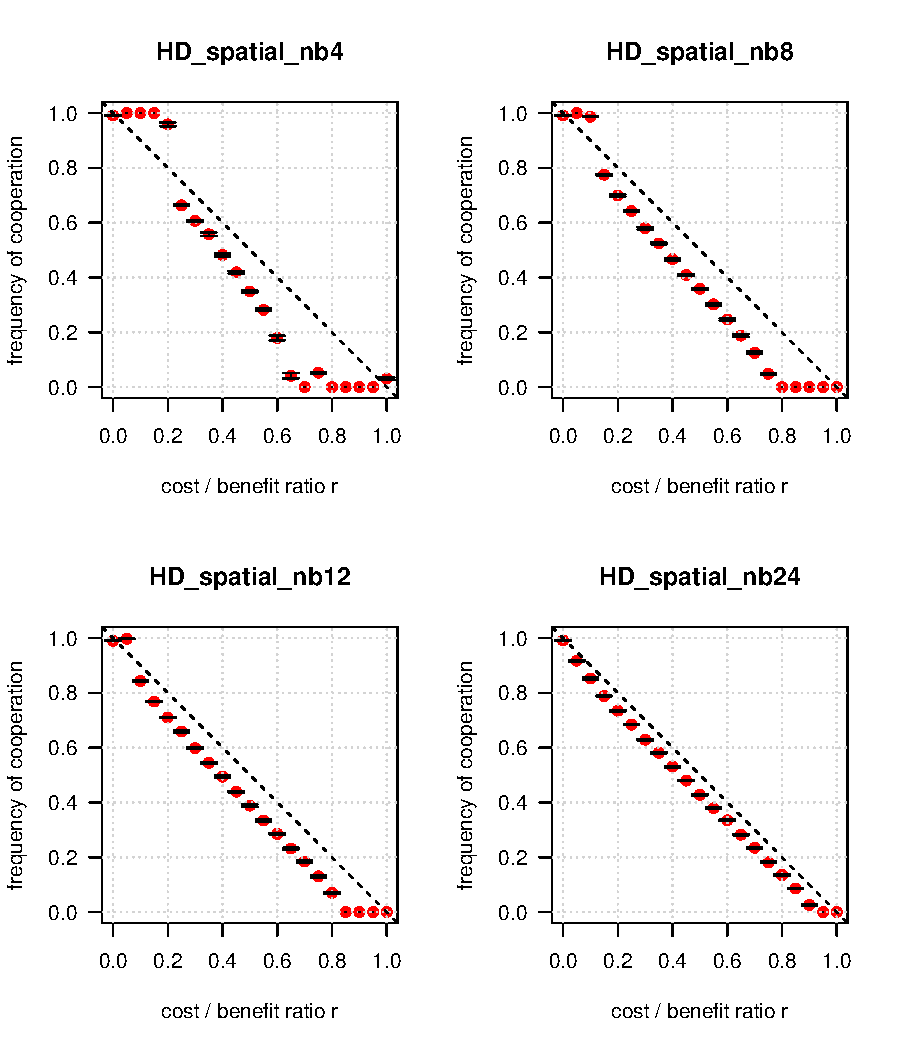
\includegraphics[width=9.5cm]{task2_4plot}
	\caption{Effect of varying neighborhood size in the HD game.  \textbf{[ t = 5000, i = 10 ]} }\label{fig: task2_4plot}
\end{figure}



\textbf{PD games} 


\begin{figure}[H]
	\centering 
	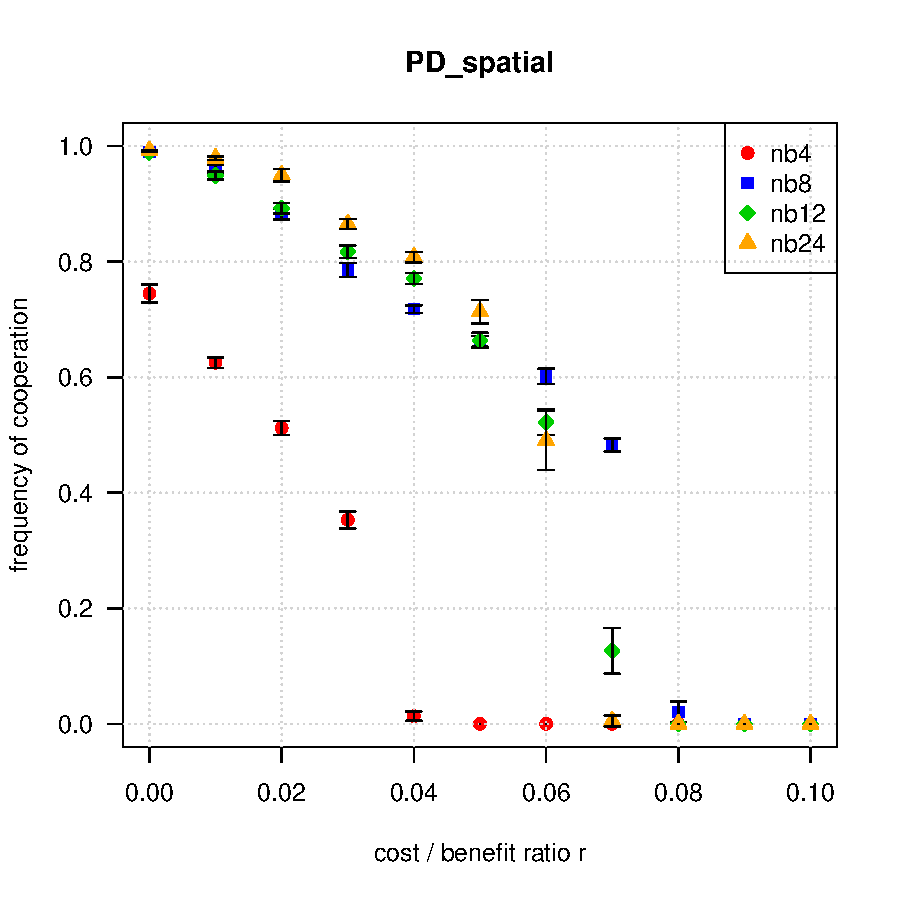
\includegraphics[width=9.5cm]{task2_multiplot}
	\caption{Spatial PD game simulations with different neighborhood sizes.  \textbf{[ t = 5000, i = 10 ]} }\label{fig: task2_multiplot}
\end{figure}


It is widely assumed that spatial structure allows for the evolution of cooperation in PD games. However, this goes only for a small range of cost-benefit ratios. Cooperation is only evolutionarily stable for r-values $ \leq 0.09$, for bigger r-values it disappears from the population.\\
 
In spatial HD games: small neighborhoods = bigger profit when r is small, and small neighborhoods = bigger disadvantage when r is big.

In spatial PD games: 


fixed r: at 0.03 and 0.065
varying neighborhood size
5000 steps, 5 repetitions

\begin{figure}[H]
	\centering 
	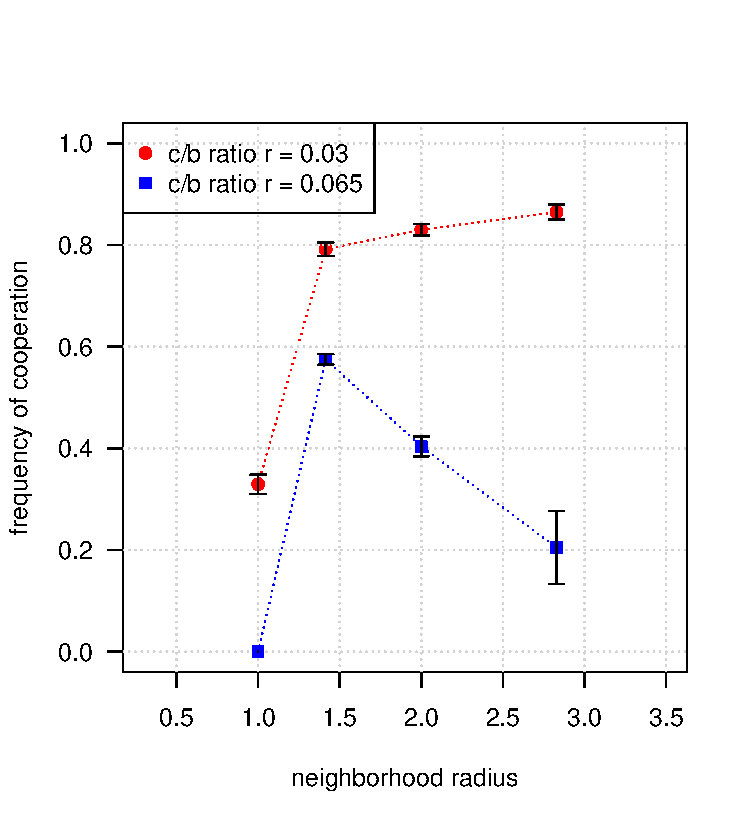
\includegraphics[width=9.5cm]{task2_radiusplot}
	\caption{Spatial PD game simulations with fixed cost-benefit-ratio and different neighborhood sizes.  \textbf{[ t = 5000, i = 10 ]} }\label{fig: task2_radiusplot}
\end{figure}


\subsection{Effect of mixed strategies}

